\documentclass{article}
\usepackage{graphicx,wrapfig,lipsum}
\usepackage[utf8]{inputenc}
\usepackage{float}

\title{Progettazione di una base di dati per esperimenti scientifici}
\author{Francesco Andreuzzi - IN0500630}
\date{\today}

\renewcommand{\figurename}{Fig.}

\begin{document}
\maketitle

Durante lo sviluppo di un progetto scientifico che comporti l'esecuzione di esperimenti di lunga durata che producano un output non banale, mantenere ordine tra i dati disponibili diventa rapidamente complesso e dispendioso in termini di tempo. Il proliferare dei metodi sperimentati (nell'\hphantom{xcjxxsksjskksksk}
\begin{wrapfigure}{r}{2cm}
    \vspace{-0.9cm}
    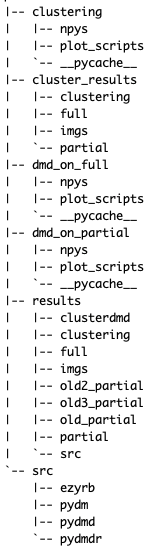
\includegraphics[width=2cm]{res/tree_brutto.png}
    \caption{\texttt{tree} della directory di un progetto.}\label{fig:tree}
\end{wrapfigure}
ambito dello stesso progetto) al fine di pervenire all'obiettivo preposto, eventualmente insieme all'aumentare del numero di parametri che controllano determinate caratteristiche degli stessi, rende la situazione ancora più caotica.  Il progetto si propone il compito di risolvere questo problema con una base di dati, al fine di evitare gerarchie di cartelle con cui risulta difficoltoso lavorare a lungo termine (come quella in Figura \ref{fig:tree}).

Il progetto sarà modelizzato nella forma di un algoritmo, che prende in input un dataset ed una n-upla di parametri, viene eseguito su un hardware di qualche tipo, e restituisce un dataset che contiene il risultato dell'esperimento. Si proverà a mantenere il più alto livello possibile di generalità, pur tentando di non ignorare dettagli importanti. Saranno fatte alcune ipotesi che, pur restringendo il campo di applicazione, sono facilmente generalizzabili e servono solamente a rendere più concreta l'esposizione.

\section{Ipotesi}
\label{sec:ipotesi}
Si supporrà che sui Cluster presi in considerazione sia installato il workload manager \texttt{Slurm}.

Gli algoritmi saranno implementati nel linguaggio Python, ed accetteranno parametri posizionali di tipo intero corrispondenti ad indici di liste definite negli stessi algoritmi. Queste saranno definite all'interno degli algoritmi in questo modo:

\verb|pod_ranks = [1-1.e-3, 1-1.e-6, 1-1.e-9, 1-1.e-12, -1]|

Ad esempio, lanciando uno script con ``\texttt{python3 script.py 2}'' si eseguirà l'algoritmo prendendo come primo parametro il terzo valore della lista \texttt{pod\_ranks}. Questa supposizione ci consente di delegare all'utente la definizione di tipi di input fantasiosi e potenzialmente non supportati dal DBMS.

\section{Schema concettuale}
% ammettiamo che una Run non ritorni un Data perchè potrebbe dare errore
\begin{figure}[H]
    \makebox[\textwidth][c]{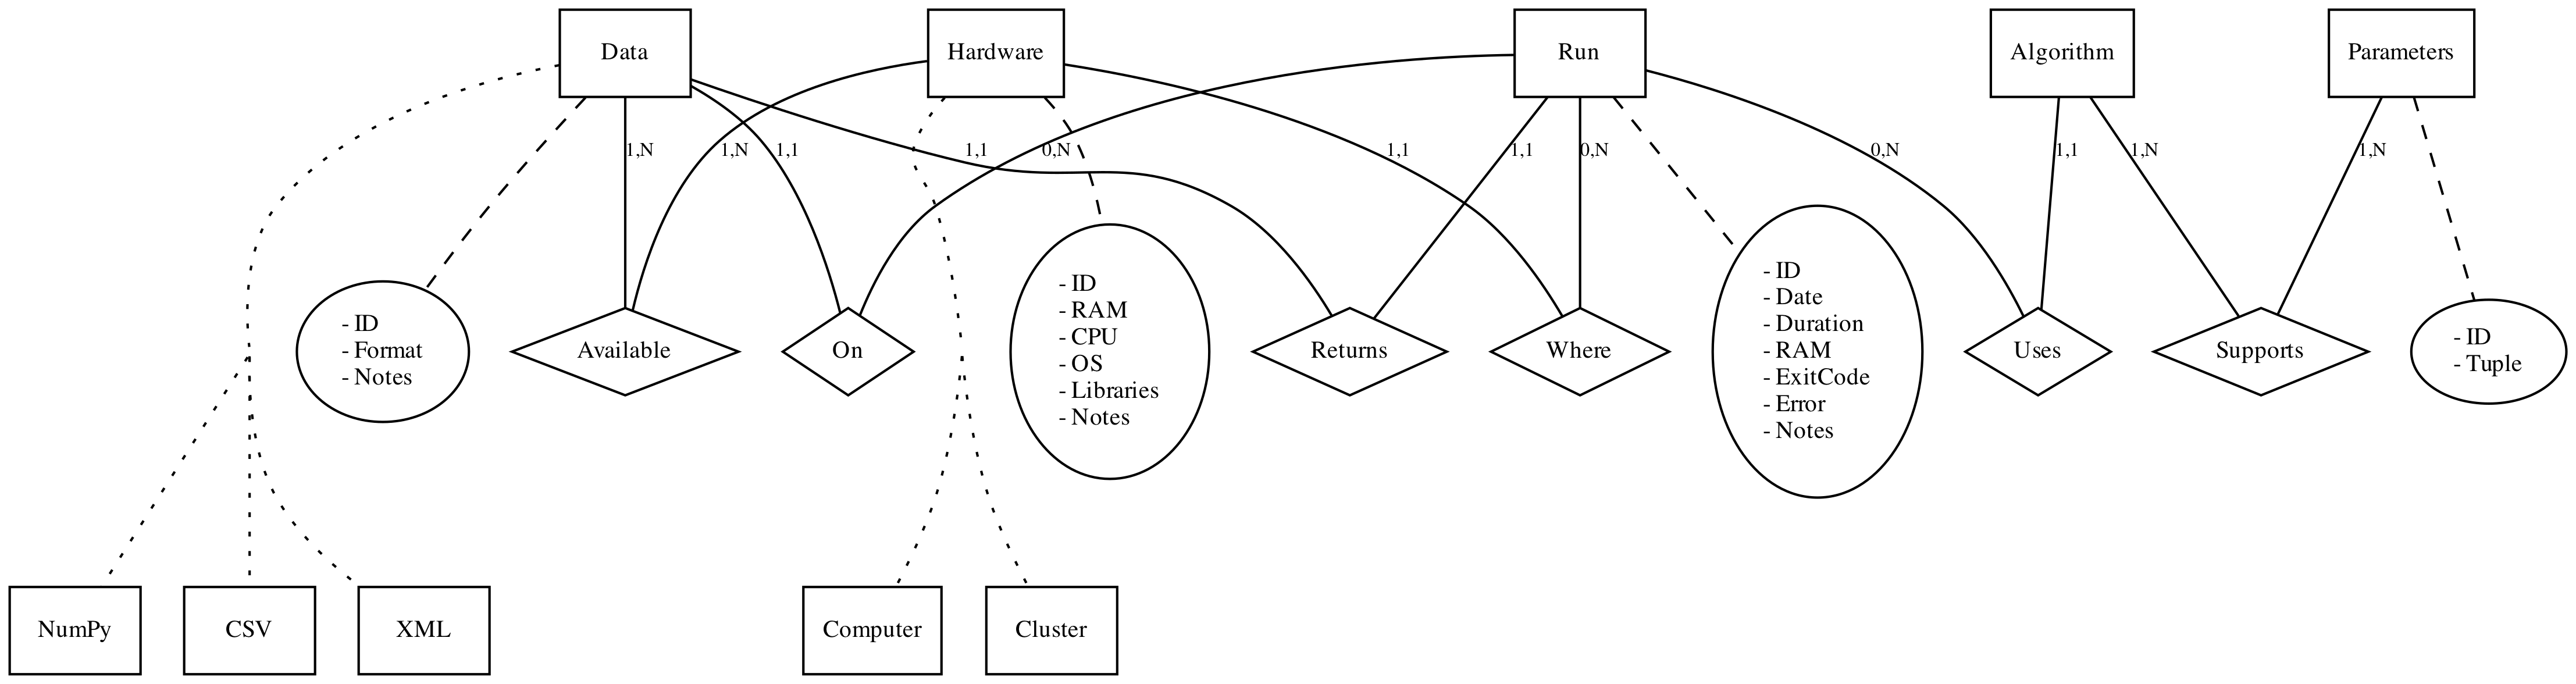
\includegraphics[width=1.6\textwidth]{res/schema_concettuale.png}}
    \caption{Schema concettuale del progetto.}
\end{figure}
Viene fornita una descrizione sintetica delle entità, delle relazioni e degli attributi.
\begin{itemize}
    \item \emph{Parameters}: Ogni riga rappresenta una tupla univoca di interi che rappresentano una possibile lista di parametri di un algoritmi, come specificato nella Sezione \ref{sec:ipotesi}. Non tutte le tuple di parametri sono supportate da tutti gli algoritmi, dato che alcuni possono richiedere un numero inferiore o superiore di parametri a seconda del metodo che implementano. Per questo motivo è stata aggiunta la relazione \emph{Supports};
    \item \emph{Algorithm}:
    \item \emph{Data}:
    \item \emph{Run}:
    \item \emph{Hardware}:
\end{itemize}

\section{Operazioni previste}
L'idea del progetto è automatizzare, eventualmente con un'interfaccia di qualche tipo oltre alla base di dati, l'intera pipeline di comandi che porta dalla situazione in cui si dispone di dataset, hardware, algoritmo e parametri, a quella in cui sono stati generati i risultati dell'esperimento corrispondente a questa 4-upla. Nel mezzo vengono dunque inglobati i seguenti compiti:
\begin{itemize}
    \item Generazione del comando per lanciare lo script in cui consiste l'esperimento, che tiene conto dei parametri e della piattaforma (nel caso di un cluster il comando sarà del tipo \texttt{sbatch ...});
    \item Scrittura dei risultati in una directory con nome dipendente da ognuno degli elementi che caratterizzano l'esperimento (algoritmo usato, parametri, hardware, dataset).
    \item Comunicazione all'utente della posizione della directory corrispondente ad una particolare n-upla algoritmo-hardware-dataset-parametri, o di una lista di directory nel caso in cui uno di questi elementi sia omesso.
\end{itemize}
Inoltre sarà necessario consentire la registrazione di nuovi algoritmi, hardware, dataset, parametri.

\section{Volumi}
\begin{table}[H]
    \begin{minipage}{.5\linewidth}
      \vspace{-1cm}
      \centering
      \begin{tabular}{||l l||}
        \hline
        Concetto & Volume \\ [0.5ex]
        \hline\hline
        Data & $<10000 + 5$\\
        Hardware & 5\\
        Run & $<10000$\\
        Algorithm & 5\\
        Parameters & 1000\\
        \hline
       \end{tabular}
    \end{minipage}
    \begin{minipage}{.5\linewidth}
      \vspace{-0.55cm}
      \centering
        \begin{tabular}{||l l||}
            \hline
            Concetto & Volume \\ [0.5ex]
            \hline\hline
            Available & $<25$\\
            On & $<10000$\\
            Returns & $<10000$\\
            Where & $<10000$\\
            Uses & $<10000$\\
            Supports & $<5000$\\
            \hline
           \end{tabular}
    \end{minipage}
\end{table}

\section{Schema logico}
Sono state rimosse le generalizzazioni totali \emph{Cluster} e \emph{Computer} di \emph{Hardware}, l'attributo \emph{Nodes} di \emph{Cluster} è accorpato a \emph{Hardware}, e vale coerentemente ``1'' se l'istanza è di tipo \emph{Computer}.

Sono state rimosse le generalizzazioni parziali di \emph{Data} in quanto la loro presenza non apportava un particolare contributo; sono state rimpiazzate dall'attributo \emph{Format}, che consente all'utente di conoscere in anticipo il formato del dataset per regolarsi di conseguenza sul metodo adeguato per aprirlo. Gli attributi \emph{Shape} e \emph{Dtype} di \emph{NumPy} possono essere ottenuti rapidamente una volta aperto il dataset (per evitare il costo del caricamento in RAM si può usare il comando \texttt{np.load(..., mmap\_mode='r')}).

E' stata rimossa l'entità \emph{Parameters}, in quanto non aveva una particolare utilità ed anzi rendeva il tutto più complicato: possiamo considerare effettivamente differenti due istanze di uno stesso algoritmo con parametri differenti, in quanto ci aspettiamo risultati del tutto indipendenti. La rimozione della relazione \emph{Supports} si può motivare in due modi:
\begin{enumerate}
    \item Costituiva un'informazione ridondante, in quanto testando una n-upla non supportata con l'algoritmo considerato si sarebbe ottenuto un errore nei primi istanti di esecuzione;
    \item L'utente può comunque indicare che una n-upla è supportata da un particolare algoritmo nel momento in cui li registra in una riga della entity \emph{Algorithms}.
\end{enumerate}
\begin{figure}[H]
    \makebox[\textwidth][c]{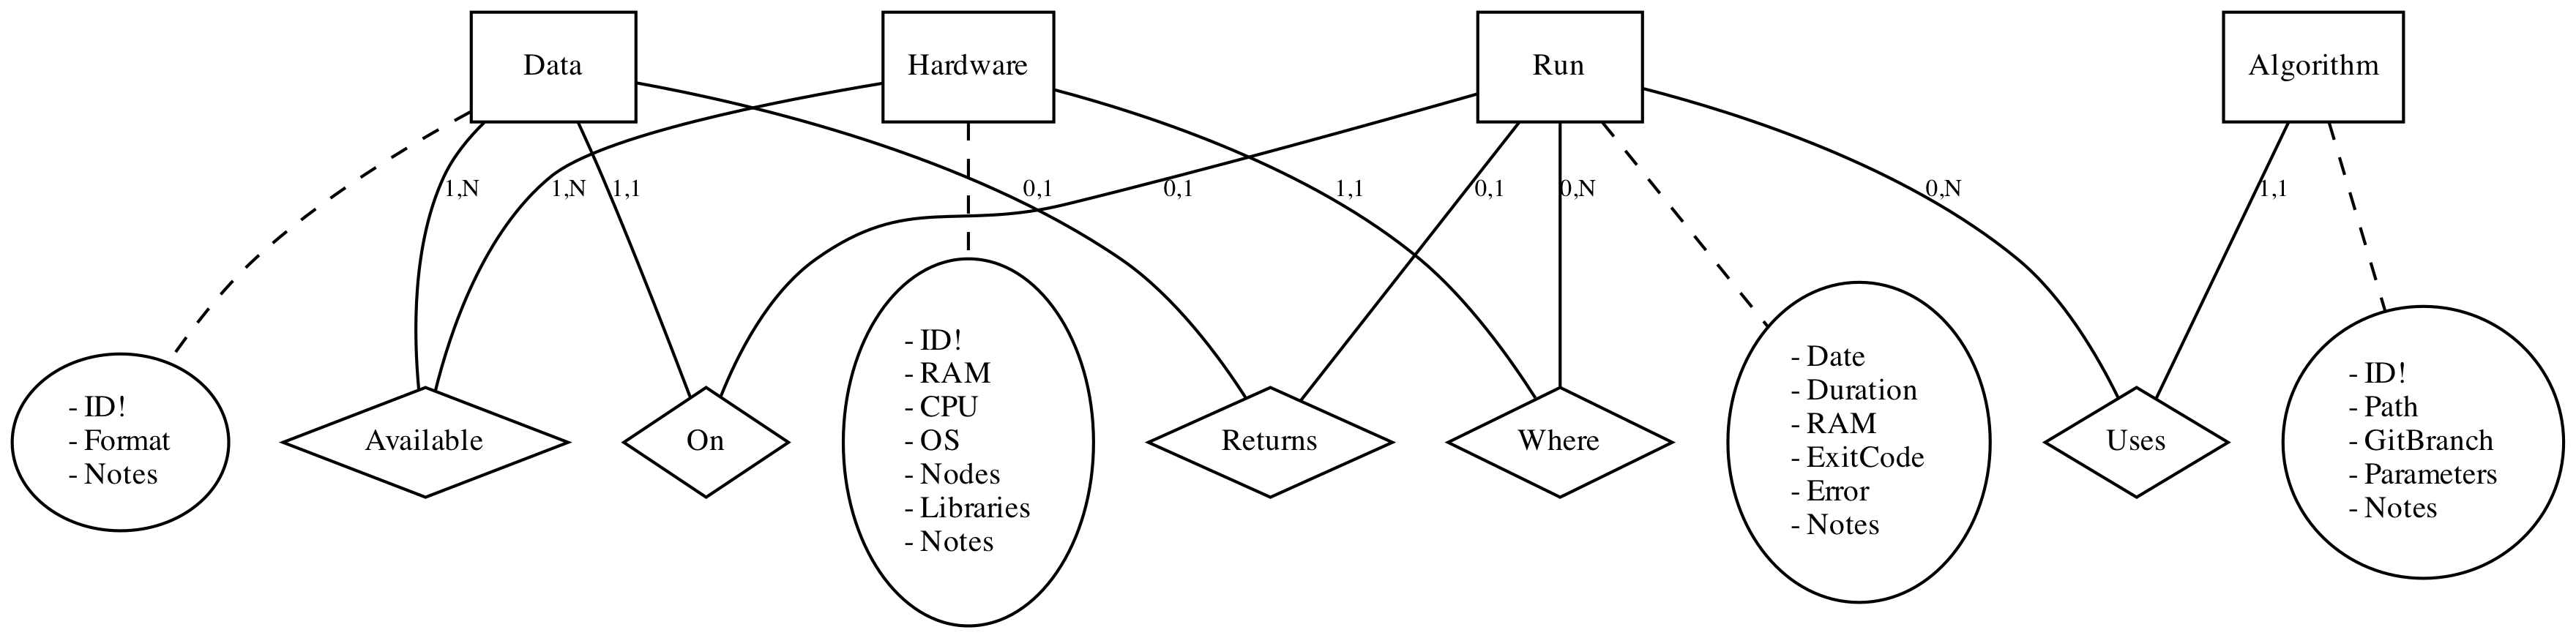
\includegraphics[width=1.6\textwidth]{res/schema_logico.png}}
    \caption{Schema logico del progetto.}
\end{figure}

\section{Note}
In un contesto più realistico l'algoritmo dovrebbe essere un eseguibile, ma linguaggi come python non funzionano così. Dovrebbe essere previsto uno script di supporto.

Questo documento è stato realizzato con \LaTeX. Gli schemi sono stati realizzati in Python utilizzando le librerie \emph{NetworkX, (Py)Graphviz}, ed il VCS \emph{git}.

L'idea per questo progetto è stata ispirata dalla collera conseguente alla necessità di dover eseguire da zero un pool di 400 \emph{jobs} sul cluster HPC della SISSA perchè i risultati corrispondenti erano stati sovrascritti da un altro esperimento con un algoritmo diverso ma parametri identici.

\end{document}
